\documentclass[11pt,a4paper]{article}
\usepackage[catalan]{babel}

% Paquetes necesarios
% preamble.tex

% Codificación y tipografía
\usepackage[utf8]{inputenc}
\usepackage[T1]{fontenc}
\usepackage[catalan]{babel}
\usepackage{lmodern}

% Márgenes y geometría
\usepackage{geometry}
\geometry{left=2.5cm, right=2.5cm, top=2cm, bottom=3cm}
% Estilo de página
\usepackage{fancyhdr}
\setlength{\headheight}{15pt}
\pagestyle{fancy}
\fancyhf{}
\lhead{\textit{Electrònica Física}}
\rhead{\textit{Adrià Rojo}}
\cfoot{\thepage}

% Gráficos y tablas
\usepackage{graphicx}
\usepackage{float}
\usepackage{caption}

% Matemáticas y símbolos
\usepackage{amsmath}
\usepackage{amssymb}

% Hipervínculos
\usepackage{hyperref}

% Espaciado
\usepackage{parskip}  % Quita sangría de párrafos y añade espacio
\usepackage{wrapfig}
\usepackage[backend=biber,style=ieee, autocite=superscript]{biblatex}
\addbibresource{bibliography.bib}

% Fuente y estilo general
\renewcommand{\familydefault}{\rmdefault}

%Definició de la ela geminada per tal que accepti el punt volat del teclat
% \def·#1{%
%   \ifmmode
%     \cdot #1
%     %\csname normal@char\string"\endcsname l%
%   \else%
%     \def\argument{#1}%
%     \if\argument l%
%       \leftllkern=0pt\rightllkern=0pt\raiselldim=0pt%
%       \setbox0\hbox{l}\setbox1\hbox{l\/}\setbox2\hbox{.}%
%       \advance\raiselldim by \the\fontdimen5\the\font
%       \advance\raiselldim by -\ht2%
%       \leftllkern=-.25\wd0%
%       \advance\leftllkern by \wd1%
%       \advance\leftllkern by -\wd0%
%       \rightllkern=-.25\wd0%
%       \advance\rightllkern by -\wd1%
%       \advance\rightllkern by \wd0%
%       \allowhyphens\discretionary{-}{l}%
%       {\hbox{}\kern\leftllkern\raise\raiselldim\hbox{.}%
%         \kern\rightllkern\hbox{l}}\allowhyphens%
%     \else
%       \if\argument L%
%         \leftllkern=0pt\rightllkern=0pt\raiselldim=0pt%
%         \setbox0\hbox{L}\setbox1\hbox{L\/}\setbox2\hbox{.}%
%         \advance\raiselldim by .5\ht0%
%         \advance\raiselldim by -.5\ht2%
%         \leftllkern=-.125\wd0%
%         \advance\leftllkern by \wd1%
%         \advance\leftllkern by -\wd0%
%         \rightllkern=-\wd0%
%         \divide\rightllkern by 6%
%         \advance\rightllkern by -\wd1%
%         \advance\rightllkern by \wd0%
%         \allowhyphens\discretionary{-}{L}%
%         {\hbox{}\kern\leftllkern\raise\raiselldim\hbox{.}%
%            \kern\rightllkern\hbox{L}}\allowhyphens%
%       \else
%         #1
%       \fi
%     \fi
%   \fi
%   }
% Título
\title{\textbf{CMOS: Història, fonaments i funcionament i aplicacions}}
\author{Adrià Rojo}
\date{\today}

\begin{document}

\maketitle
\thispagestyle{fancy}
% Resumen
\begin{abstract}
    BLABLA
\end{abstract}

\section{Introducció}
% Introducir brevemente qué es CMOS, su importancia en la electrónica digital y qué estructura tendrá el trabajo.

Un semiconductor-òxid-metall complementari (\textit{Complementary-Metal-Oxide Semiconductor}) és un tipus de tecnologia que combina un parell simètric de N-MOS i P-MOS conectats de forma complementària per poder fer operacions lògiques de forma eficient \autocite{wiki:CMOS}. 

Aquesta tecnologia és la base d'electrònica moderna, sent el bloc principal de la porta lògica \texttt{NAND}, que és la base de tots els altres circuits existents i pot arribar formar circuits molt complexos com processadors i memòries RAM.

Els dispositius dissenyats amb el procés CMOS en ment també poden ser utilitzats com a sensor d'imatge, gràcies a la seva eficiència i rapidesa, format part d'una àmplia varietat d'eines electròniques, des de telèfons mòbils a drons i càmeres fotogràfiques utilitzades en medicina o astronomia. 

Actualment s'estima que el nombre de transistors fabricats (CMOS i altres MOS) superen els $10^{22}$ dispositius el 2018 \autocite{wiki:Transistor_count}, dada que està basada en la Llei de Moore.

A continuació, parlarem sobre la història de la tecnologia CMOS, els principis físics, el seu funcionament intern i les seves aplicacions actuals i futures.

\begin{figure}[h]
    \centering
    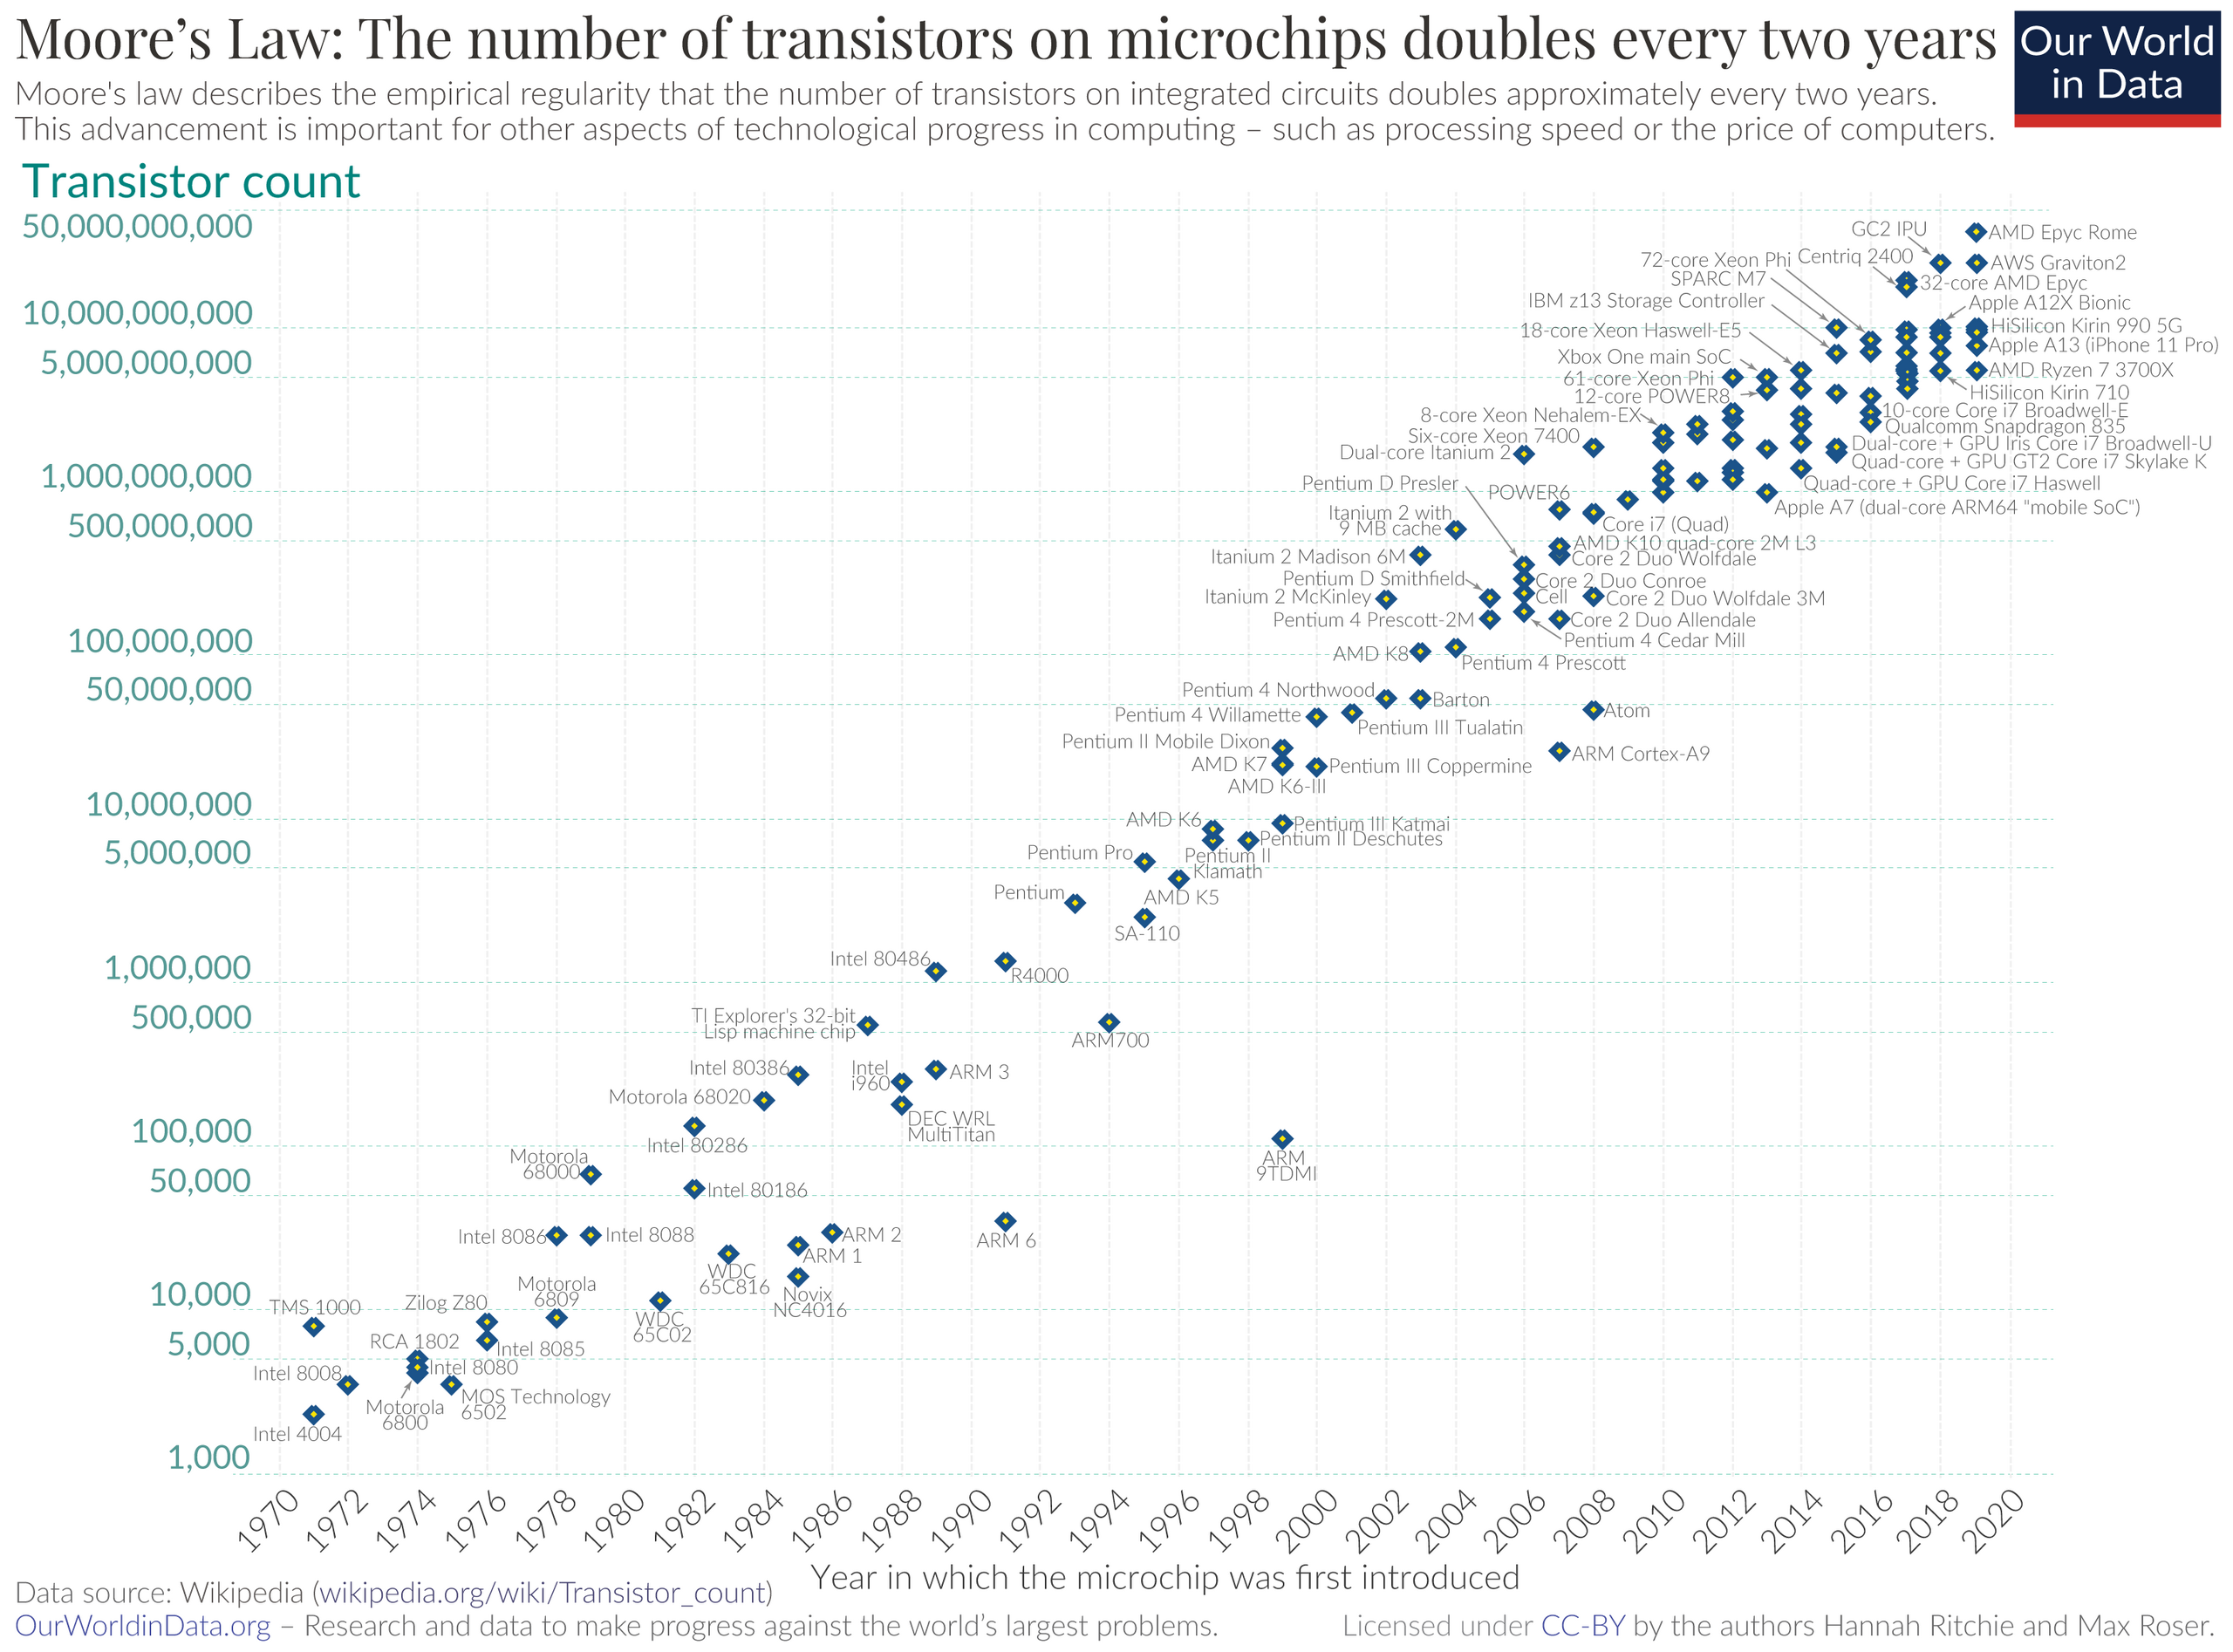
\includegraphics[width=0.6\linewidth]{Moore's_Law_Transistor_Count_1970-2020.png}
    \caption{Gràfic de quantitat de transistors MOS per any. Wikipedia.}
    \label{<label>}
\end{figure}

\section{Història del CMOS}
% Destacar los hitos importantes desde 1963, comparaciones con tecnologías anteriores (NMOS, BJT).
% Mencionar su adopción masiva en los años 80-90 y cómo ha evolucionado.

\section{Funcionament intern}

\subsection{Estructura d'un CMOS}
% Describir un inversor básico nMOS/pMOS en serie con explicación de entrada/salida.

\subsection{Bandes d'energia}
% Explicar las bandas de valencia/conducción en nMOS y pMOS, con comentario sobre inversión de canal.
% Comentar brevemente el modelo de portadores mayoritarios.

\subsection{Corrent de portadors}
% Diferenciar entre flujo de electrones (nMOS) y huecos (pMOS). 
% Mencionar el principio de conducción dependiente del voltaje de puerta.

% \subsection{Consumo de Potencia}
% % Diferenciar entre consumo estático y dinámico.
% % Comentar sobre la eficiencia del CMOS frente a otras tecnologías.

\section{Aplicacions}

\subsection{Portes lògiques}

\subsection{Sensors i cameres digitals}
% Cámaras digitales, sensores industriales, robótica.

\printbibliography

\end{document}
